\visible<1->{A neural network (NN) takes an initial representation as an input.}\\
\visible<2->{Hidden layers in the NN utilize distort the representation in a high dimensional space, thus learning a new representation. This separation allows ease of classification or regression}\\
\begin{tikzpicture}[shorten >=1pt,draw=black, x=1cm, y=1 cm,  node distance=0cm]
	\draw[draw=gray, use as bounding box](-2,0) rectangle (8,6);
	\clip (-2,-0) rectangle (8,6);
	\def\layersep{2cm}
	
	\tikzstyle{every pin edge}=[<-,shorten <=1pt,thick]
	\tikzstyle{neuron}=[circle,fill=black!25,minimum size=0.5cm ,inner sep=0pt, color=black, draw]
	\tikzstyle{input neuron}=[neuron, fill=green!50!blue!50];
	\tikzstyle{output neuron}=[neuron, fill=green!50!blue];
	\tikzstyle{hidden neuron}=[neuron, fill=green!50!orange];
	\tikzstyle{annot} = [text width=2em, text centered]

	\visible<3->{\node[black,thick,minimum width = 8cm,minimum height = 8cm,path picture={\node at (path picture bounding box.center){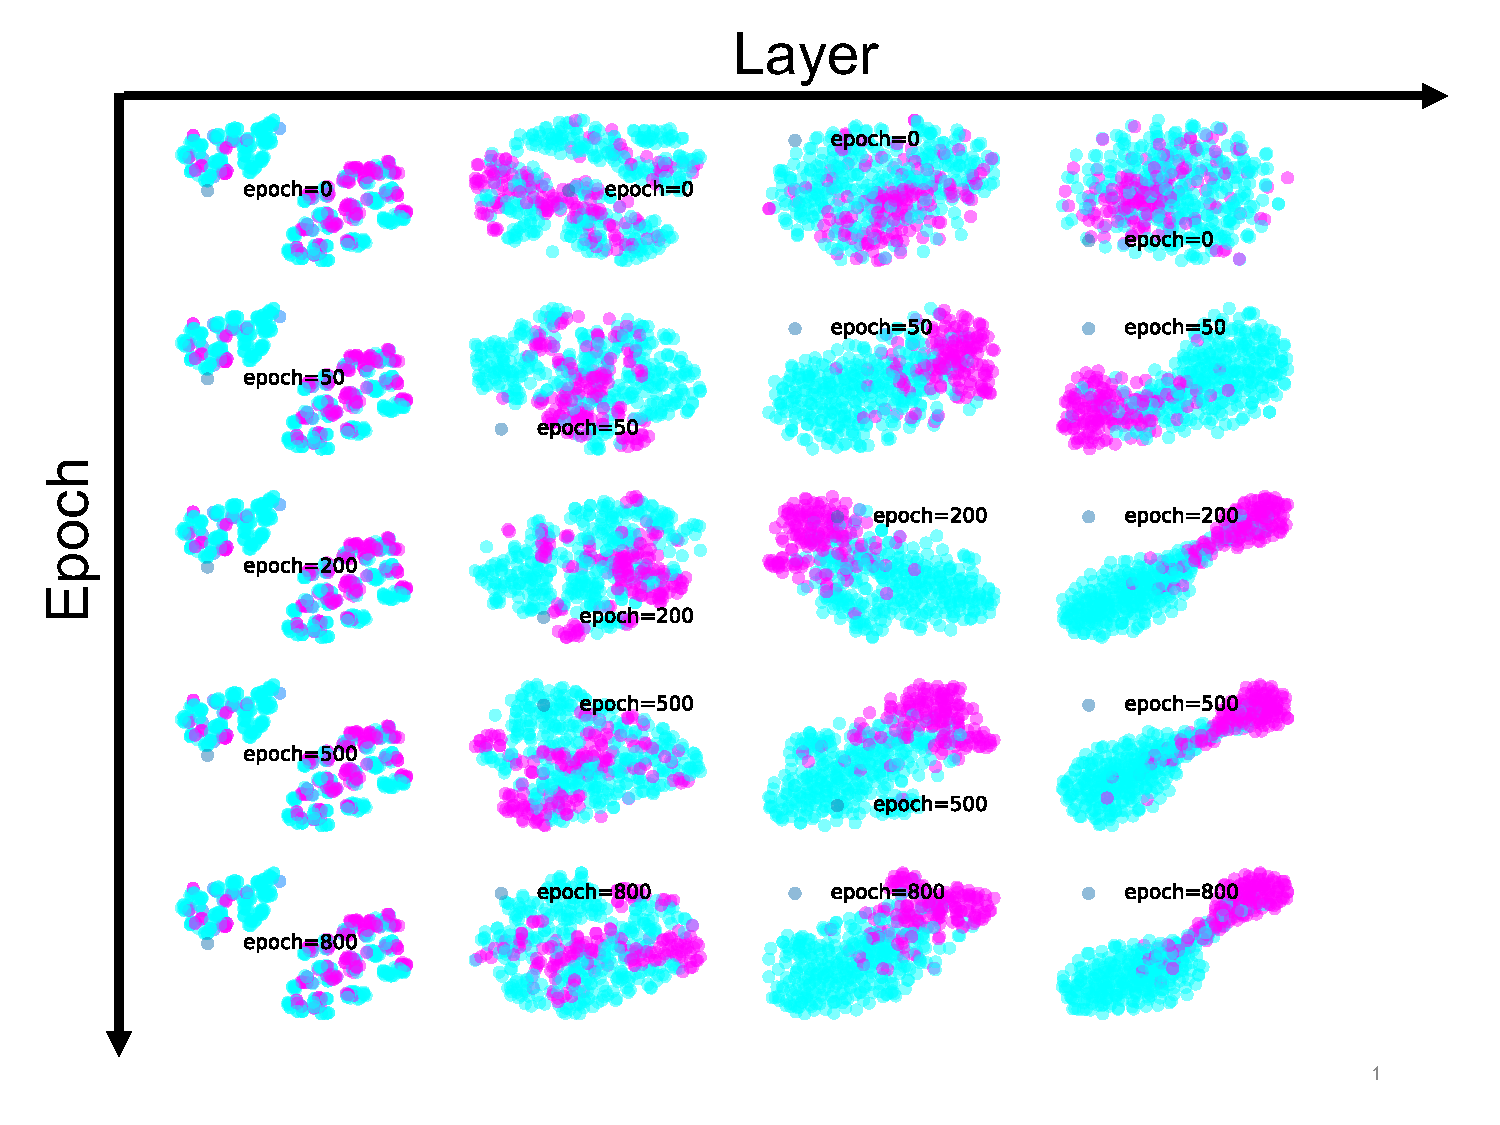
\includegraphics[width=8cm]{neural_networks/images/rep_learning}}; }] (Xp) at (3,3) {};}
\end{tikzpicture}
